\chapter{Experiments}
\label{ch:experiments}

% \todo{Add trees depth for all tables. White about users == annotators}

We conducted a series of experiments to study the impact of adding vector words' representations as features for a classification model on the quality of the words' categorization. As in this work we compare results with ones in \citep{Grabar-PITR2014}, we first, reproduce results from the paper on the same datasets. Then we check how FastText word embeddings influence the quality of classification in different cross-validation scenarios. We notice that in one scenario FastText word embeddings significantly and confidently improve the performance of the classification model, so the next step is to study whether this model generalizes well on a greater variety of users. Finally, we study how FrnnMUTE used as features impact on classification quality in all the same cross-validation scenarios as considered previously and on all available user annotations.

\section{Reproduction of previous results}

In \citep{Grabar-PITR2014} the classification methods were obtained using WEKA\footnote{\url{https://www.cs.waikato.ac.nz/ml/weka/}} - a collection of machine learning algorithms for data mining tasks implemented on Java. In our research as a tool to conduct experiments, we used Python as there are a lot of stable third-party Python libraries that make it convenient for research. In order to ensure the consistency of experiments in this work and in \citep{Grabar-PITR2014}, firstly, we reproduced the results in WEKA using the pre-computed set of standard features described in the previous section \ref{sec:standard-features} and \textit{J48} classification algorithm - a WEKA implementation of C4.5 decision tree based algorithm described in \cite{Quinlan1993}. Our results perfectly match with ones presented in the paper. 

Secondly, we developed a solution in Python based on DT classifier from well-known scikit-learn library\footnote{\url{http://scikit-learn.org}}. At this step we got 0.85-1.41 lower $F$ scores for scikit-learn classifier compared to WEKA results (Table \ref{tab:results-reproduction}).

\begin{table*}[h]
\begin{tabular}{L|LLL}
\hline
\textit{user \textbackslash method} & \textit{Results from paper \citep{Grabar-PITR2014}} & \textit{WEKA J48} & \textit{Python Decision trees (10-fold CV, with shuffle)} \\ \hline
$O1$ & 80.6 & 80.5 & 79.8 \\
$O2$ & 81.4 & 80.9 & 80.0 \\
$O3$ & 84.5 & 84.5 & 83.2 \\ \hline
\end{tabular}
    \caption{Comparison of different implementations of a decision tree classifier on three sets of annotations (O1, O2, O3) in user-in vocabulary-out cross-validation. The DT in scikit-learn was restricted to depth not more than 3 (this showed the best result during grid-search of hyperparameters of the DT).}
    \label{tab:results-reproduction}
\end{table*}

Since the input features were identical for both of WEKA and scikit-learn frameworks, we concluded that the little degradation of quality in case of using scikit-learn is caused by the difference in implementations of decision tree classifiers in these frameworks. In all subsequent experiments, we will use a scikit-learn classification DT model for convenient experiments' results comparison. We will introduce slight changes in depth of a DT for different dimensions of feature sets.


\section{Experiments with cross-validation scenarios}
\label{sec:cv-experiments}
\subsection{User-in vocabulary-out cross-validation}

% These experiments also follow the scenario from \cite{Grabar-PITR2014}. The cross-validation is done on each dataset (i.e. each user's annotation) separately. The goal of these experiments is to measure the ability of the method to generalize class recognition on the \textit{known user} and his known manner to annotate words (that is, his understanding of the meaning of medical words) for \textit{unknown words}. 

We carried out the experiments using (i) the standard features only, (ii) the FastText word embeddings only and (iii) their combination. Experiments with isolated FastText word embeddings as features and the data from three annotators resulted in poor F1 scores (Table \ref{tab:user-in-voc-out}), that can be treated that contextual information which is dominant in the word embeddings is not enough to define the word understandability. Adding the FastText word embeddings to the standard feature set resulted in up to 1.0 higher F1 score due to higher Precision (up to 1.8), meaning that contextual information slightly impacts on the understandability of a word by a given person.

\begin{table*}[h]
\begin{tabular}{cc|cccc|cccc|cccc}
\multirow{2}{0.6cm}{\textit{Train user}} & \multirow{2}{0.6cm}{\textit{Test user}} & \multicolumn{4}{c|}{\textit{Standard features}} & \multicolumn{4}{c|}{\textit{FastText embeddings}} & \multicolumn{4}{X}{\textit{Standard features + FastText embeddings}} \\ \cline{3-14} 
 &  & $A$ & $P$ & $R$ & $F$ & $A$ & $P$ & $R$ & $F$ & $A$ & $P$ & $R$ & $F$ \\ \hline
$O1$ & $O1$ & \textbf{82.5} & 77.2 & \textbf{82.5} & 79.8 & 72.5 & 67 & 72.5 & 69.3 & 82.4 & \textbf{79} & 82.4 & \textbf{80.2} \\
$O2$ & $O2$ & \textbf{82} & 78.9 & \textbf{82} & 80 & 73.5 & 69.9 & 73.5 & 71.3 & 81.9 & \textbf{79.5} & 81.9 & \textbf{80.3} \\ 
$O3$ & $O3$ & 85.5 & 81.2 & 85.5 & 83.2 & 74.9 & 70.4 & 74.9 & 72.3 & \textbf{85.9} & \textbf{83} & \textbf{85.9} & \textbf{84.2} \\ \hline 
\end{tabular}
    \caption{Experiments on user-in vocabulary-out cross-validation. The best score for a combination of quality measure and experiment among three feature sets is in bold.}
    \label{tab:user-in-voc-out}
\end{table*}


\subsection{User-out vocabulary-in cross-validation}

% In this setting, we measure the ability of the classifier to generalize on all known words, but for unknown users (Table \ref{tab:user-out-voc-in}). This scenario is realistic to a real-world situation: the reference annotations can be obtained only from a couple of users, presumably representing the overall population, but not from all the possible users. Yet, it is necessary to predict the familiarity of medical words for all the potential users even if they did not participate in the annotations.

In these experiments we got a significant\todo{ngr: important or statistically significant?} improvement of combined features in comparison to the standard features (Table \ref{tab:user-out-voc-in}). When knowledge of words understandability of one user is used to predict it for another user, adding the FastText word embeddings provides up to 2.9 better F1 score. Notice that used separately, standard features and embeddings show similar performance as in user-in vocabulary-out cross-validation (Table \ref{tab:user-in-voc-out}). Our hypothesis is that there exists a robust nonlinear dependency between some subsets of standard features and subword-level components of FastText word embeddings. Testing this hypothesis is the topic of our further research.

\begin{table*}[h]
\begin{tabular}{cc|cccc|cccc|cccc}
\multirow{2}{0.6cm}{\textit{Train user}} & \multirow{2}{0.6cm}{\textit{Test user}} & \multicolumn{4}{c|}{\textit{Standard features}} & \multicolumn{4}{c|}{\textit{FastText embeddings only}} & \multicolumn{4}{X}{\textit{Standard features + FastText embeddings}} \\ \cline{3-14} 
 &  & $A$ & $P$ & $R$ & $F$ & $A$ & $P$ & $R$ & $F$ & $A$ & $P$ & $R$ & $F$ \\ \hline
\textit{O1} & \textit{O2} & 81.7 & 78.6 & 81.7 & 80.1 & 74 & 70.3 & 74 & 71.2 & \textbf{84.2} & \textbf{82} & \textbf{84.2} & \textbf{82.8} \\  
\textit{O1} & \textit{O3} & 85 & 81.2 & 85 & 83 & 75.4 & 70.7 & 75.4 & 72.6 & \textbf{87.6} & \textbf{84.9} & \textbf{87.6} & \textbf{85.9} \\ \hline 
\textit{O2} & \textit{O1} & 82.2 & 77 & 82.2 & 79.1 & 72.8 & 67.3 & 72.8 & 69.6 & \textbf{83.9} & \textbf{80.2} & \textbf{83.9} & \textbf{81.1} \\  
\textit{O2} & \textit{O3} & 85.4 & 81.1 & 85.4 & 83 & 75.3 & 71.1 & 75.3 & 73 & \textbf{86.8} & \textbf{83.5} & \textbf{86.8} & \textbf{84.7} \\ \hline 
\textit{O3} & \textit{O1} & 82.8 & 77.4 & 82.8 & 79.7 & 72.7 & 67.1 & 72.7 & 69.4 & \textbf{84.9} & \textbf{81.3} & \textbf{84.9} & \textbf{82.4} \\  
\textit{O3} & \textit{O2} & 82.2 & 79 & 82.2 & 80.2 & 74.1 & 70.4 & 74.1 & 71.6 & \textbf{84.2} & \textbf{82.1} & \textbf{84.2} & \textbf{82.8} \\ \hline 
\end{tabular}
    \caption{Experiments on user-out vocabulary-in cross-validation.}
    \label{tab:user-out-voc-in}
\end{table*}


\subsection{User-out vocabulary-out cross-validation}
\label{sec:user-out-voc-out}

The cross-validation setting is now the most strict and knowledge of words understandability of one user is used to predict whether another user will understand other medical words. In these experiments, FastText word embeddings provide approximately 0.5\% higher F1 score in case of learning on users O1 and O3 (Table \ref{tab:user-out-voc-out}). When learning on user O2, embeddings decrease F by 0.5, which means that annotations and health literacy of user O2 are different from users O1 and O3. It seems that adding embeddings makes overfitting of machine learning model to the dataset. As a result, tests on other "kind of word understandability" and on combined features are less successful compared to using standard features only for learning. This may be due to the lack of systematicity in annotations of O2. We will also encounter this issue when more annotators are involved in experiments in sections \ref{sec:generalizability-study} and \ref{sec:frnnmute-study}.

\begin{table*}[h]
\begin{tabular}{cc|cccc|cccc|cccc}
\multirow{2}{0.6cm}{\textit{Train user}} & \multirow{2}{0.6cm}{\textit{Test user}} & \multicolumn{4}{c|}{\textit{Standard features}} & \multicolumn{4}{c|}{\textit{FastText embeddings}} & \multicolumn{4}{X}{\textit{Standard features + FastText embeddings}} \\ \cline{3-14} 
 &  & $A$ & $P$ & $R$ & $F$ & $A$ & $P$ & $R$ & $F$ & $A$ & $P$ & $R$ & $F$ \\ \hline
\textit{O1} & \textit{O2} & 81.7 & 78.6 & 81.7 & 80.1 & 73.6 & 69.9 & 73.6 & 71.3 & \textbf{81.8} & \textbf{79.8} & \textbf{81.8} & \textbf{80.6} \\ 
\textit{O1} & \textit{O3} & \textbf{85} & 81.2 & \textbf{85} & 83 & 74.8 & 70.4 & 74.8 & 72.4 & 84.9 & \textbf{82.2} & 84.9 & \textbf{83.4} \\ \hline 
\textit{O2} & \textit{O1} & \textbf{82.2} & 76.9 & \textbf{82.2} & \textbf{79.1} & 72.5 & 66.9 & 72.5 & 69.3 & 81.7 & \textbf{77.5} & 81.7 & \textbf{79.1} \\
\textit{O2} & \textit{O3} & \textbf{85.3} & 81 & \textbf{85.3} & \textbf{83} & 75.1 & 70.7 & 75.1 & 72.7 & 84.4 & \textbf{81.3} & 84.4 & 82.5 \\ \hline 
\textit{O3} & \textit{O2} & \textbf{82.7} & 77.3 & \textbf{82.7} & 79.7 & 72.5 & 66.9 & 72.5 & 69.2 & 82.6 & \textbf{78.9} & 82.6 & \textbf{80.2} \\ 
\textit{O3} & \textit{O3} & 82.1 & 79 & 82.1 & 80.1 & 73.8 & 70.2 & 73.8 & 71.4 & \textbf{82.2} & \textbf{80} & \textbf{82.2} & \textbf{80.7} \\ \hline 
\end{tabular}
    \caption{Experiments on user-out vocabulary-out cross-validation.}
    \label{tab:user-out-voc-out}
\end{table*}

\section{Generalizability study}
\label{sec:generalizability-study}
In the previous experiments, we concentrated on three annotators' data to be consistent with the research in paper \citep{Grabar-PITR2014}. To study better generalizability of models for words' understandability detection, we included four more annotators in an experiment.

In this part, we concentrated on the user-out vocabulary-in cross-validation scenario as the most realistic one. Here understanding of the quality of generalization is crucial for usage of the model in real world client-doctor relationship.

\begin{table*}
  \centering
  \begin{tabular}{c|c|c|c|c||c|c|c||c|c|c}
    \multirow{2}{0.6cm}{\textit{Train user}} & \multirow{2}{0.6cm}{\textit{Test user}}  & \multicolumn{3}{L||}{\it Standard features} & \multicolumn{3}{L||}{\it FastText embeddings} & \multicolumn{3}{L}{\it Standard features + FastText emb}\\ \cline{3-11}
  &  & $P$ & $R$ & $F$ & $P$ & $R$ & $F$ & $P$ & $R$ & $F$
  \\ \hline
$O1$&$O1$&\he{77.2}&\he{82.5}&\he{79.7}&\he{67.0}&\he{72.5}&\he{69.3}&\he{79.0}&\he{82.4}&\he{80.2}\\
$O1$&$O2$&\he{78.6}&\he{81.7}&\he{80.1}&\he{70.3}&\he{74.0}&\he{71.2}&\he{82.0}&\he{84.2}&\he{82.8}\\
$O1$&$O3$&\he{81.2}&\he{85.0}&\he{83.0}&\he{70.7}&\he{75.4}&\he{72.6}&\he{84.9}&\he{87.6}&\he{85.9}\\
$O1$&$A1$&\he{71.0}&\he{74.7}&\he{71.2}&\he{62.1}&\he{63.8}&\he{58.8}&\he{74.1}&\he{75.4}&\he{72.2}\\
$O1$&$A2$&\he{70.6}&\he{78.4}&\he{74.0}&\he{61.9}&\he{68.5}&\he{63.3}&\he{75.0}&\he{80.1}&\he{76.2}\\
$O1$&$A7$&\he{72.6}&\he{77.5}&\he{74.2}&\he{63.0}&\he{66.6}&\he{61.9}&\he{76.2}&\he{78.9}&\he{75.8}\\
$O1$&$A8$&\he{82.3}&\he{84.9}&\he{83.5}&\he{73.1}&\he{76.8}&\he{74.5}&\he{85.7}&\he{87.8}&\he{86.6}\\
\hline
$O2$&$O1$&\he{77.0}&\he{82.2}&\he{79.1}&\he{67.3}&\he{72.8}&\he{69.6}&\he{80.2}&\he{83.9}&\he{81.1}\\
$O2$&$O2$&\he{78.9}&\he{82.0}&\he{80.0}&\he{69.9}&\he{73.5}&\he{71.3}&\he{79.5}&\he{81.9}&\he{80.3}\\
$O2$&$O3$&\he{81.1}&\he{85.4}&\he{83.0}&\he{71.1}&\he{75.3}&\he{73.0}&\he{83.5}&\he{86.8}&\he{84.7}\\
$O2$&$A1$&\he{71.1}&\he{72.1}&\he{68.2}&\he{61.7}&\he{64.5}&\he{60.2}&\he{74.0}&\he{75.1}&\he{71.5}\\
$O2$&$A2$&\he{70.8}&\he{77.3}&\he{72.7}&\he{61.8}&\he{68.9}&\he{64.2}&\he{76.0}&\he{79.8}&\he{75.5}\\
$O2$&$A7$&\he{72.7}&\he{75.6}&\he{71.8}&\he{62.6}&\he{67.0}&\he{62.8}&\he{75.9}&\he{78.3}&\he{74.9}\\
$O2$&$A8$&\he{83.0}&\he{86.2}&\he{84.4}&\he{73.7}&\he{77.1}&\he{75.3}&\he{85.4}&\he{88.2}&\he{86.7}\\
\hline
$O3$&$O1$&\he{77.4}&\he{82.8}&\he{79.7}&\he{67.1}&\he{72.7}&\he{69.4}&\he{81.3}&\he{84.9}&\he{82.4}\\
$O3$&$O2$&\he{79.0}&\he{82.2}&\he{80.2}&\he{70.4}&\he{74.1}&\he{71.6}&\he{82.1}&\he{84.2}&\he{82.8}\\
$O3$&$O3$&\he{81.2}&\he{85.5}&\he{83.2}&\he{70.4}&\he{74.9}&\he{72.3}&\he{83.0}&\he{85.9}&\he{84.2}\\
$O3$&$A1$&\he{71.8}&\he{73.3}&\he{69.5}&\he{61.7}&\he{64.1}&\he{59.6}&\he{75.1}&\he{75.4}&\he{72.1}\\
$O3$&$A2$&\he{71.2}&\he{78.0}&\he{73.5}&\he{61.8}&\he{68.7}&\he{63.9}&\he{76.8}&\he{80.2}&\he{76.3}\\
$O3$&$A7$&\he{73.2}&\he{76.5}&\he{72.9}&\he{62.4}&\he{66.6}&\he{62.2}&\he{77.2}&\he{78.8}&\he{75.8}\\
$O3$&$A8$&\he{82.6}&\he{85.8}&\he{84.1}&\he{73.7}&\he{77.2}&\he{75.2}&\he{86.0}&\he{88.0}&\he{86.9}\\
\hline
$A1$&$O1$&\he{77.2}&\he{82.5}&\he{79.8}&\he{66.5}&\he{67.9}&\he{66.6}&\he{76.9}&\he{79.5}&\he{77.6}\\
$A1$&$O2$&\he{78.6}&\he{81.6}&\he{80.1}&\he{69.2}&\he{69.0}&\he{68.5}&\he{78.8}&\he{79.6}&\he{78.9}\\
$A1$&$O3$&\he{81.2}&\he{84.9}&\he{82.9}&\he{70.7}&\he{69.6}&\he{69.2}&\he{81.8}&\he{82.0}&\he{81.0}\\
$A1$&$A1$&\he{70.9}&\he{74.7}&\he{71.3}&\he{59.4}&\he{64.6}&\he{61.8}&\he{72.4}&\he{75.1}&\he{72.9}\\
$A1$&$A2$&\he{70.5}&\he{78.3}&\he{74.0}&\he{60.6}&\he{66.4}&\he{63.2}&\he{73.7}&\he{78.6}&\he{75.0}\\
$A1$&$A7$&\he{72.6}&\he{77.5}&\he{74.2}&\he{61.3}&\he{66.1}&\he{63.6}&\he{75.1}&\he{79.2}&\he{76.5}\\
$A1$&$A8$&\he{82.2}&\he{84.8}&\he{83.5}&\he{72.3}&\he{70.4}&\he{70.4}&\he{81.5}&\he{81.0}&\he{80.5}\\
\hline
$A2$&$O1$&\he{77.3}&\he{82.6}&\he{79.8}&\he{67.2}&\he{72.6}&\he{69.6}&\he{81.0}&\he{82.8}&\he{81.8}\\
$A2$&$O2$&\he{78.6}&\he{81.6}&\he{80.1}&\he{70.4}&\he{74.0}&\he{71.9}&\he{82.0}&\he{82.0}&\he{82.0}\\
$A2$&$O3$&\he{81.2}&\he{84.9}&\he{83.0}&\he{71.0}&\he{75.2}&\he{73.0}&\he{84.9}&\he{85.4}&\he{85.1}\\
$A2$&$A1$&\he{70.9}&\he{74.6}&\he{71.2}&\he{61.5}&\he{64.6}&\he{60.4}&\he{76.5}&\he{76.5}&\he{74.7}\\
$A2$&$A2$&\he{70.6}&\he{78.4}&\he{74.0}&\he{61.2}&\he{68.4}&\he{63.7}&\he{74.7}&\he{77.8}&\he{75.6}\\
$A2$&$A7$&\he{72.6}&\he{77.5}&\he{74.2}&\he{62.4}&\he{67.0}&\he{63.0}&\he{77.6}&\he{78.9}&\he{77.3}\\
$A2$&$A8$&\he{82.2}&\he{84.8}&\he{83.4}&\he{73.8}&\he{77.0}&\he{75.3}&\he{85.6}&\he{85.3}&\he{85.4}\\
\hline
$A7$&$O1$&\he{77.1}&\he{82.5}&\he{79.7}&\he{67.6}&\he{73.2}&\he{69.9}&\he{79.4}&\he{81.9}&\he{80.3}\\
$A7$&$O2$&\he{78.5}&\he{81.6}&\he{80.0}&\he{70.6}&\he{74.2}&\he{71.8}&\he{80.6}&\he{81.4}&\he{80.9}\\
$A7$&$O3$&\he{81.0}&\he{84.9}&\he{82.9}&\he{71.3}&\he{75.7}&\he{73.3}&\he{83.1}&\he{83.8}&\he{83.0}\\
$A7$&$A1$&\he{71.0}&\he{74.4}&\he{70.9}&\he{62.1}&\he{64.8}&\he{60.3}&\he{75.8}&\he{78.0}&\he{75.7}\\
$A7$&$A2$&\he{70.5}&\he{78.2}&\he{73.8}&\he{62.0}&\he{69.1}&\he{64.3}&\he{75.3}&\he{79.6}&\he{76.5}\\
$A7$&$A7$&\he{72.6}&\he{77.4}&\he{74.0}&\he{62.2}&\he{67.0}&\he{63.1}&\he{74.5}&\he{77.5}&\he{75.3}\\
$A7$&$A8$&\he{81.9}&\he{84.7}&\he{83.3}&\he{73.7}&\he{77.2}&\he{75.3}&\he{82.8}&\he{82.7}&\he{82.4}\\
\hline
$A8$&$O1$&\he{77.0}&\he{82.4}&\he{79.6}&\he{67.2}&\he{72.7}&\he{69.6}&\he{80.8}&\he{84.4}&\he{81.7}\\
$A8$&$O2$&\he{78.4}&\he{81.5}&\he{79.8}&\he{70.4}&\he{74.0}&\he{71.7}&\he{82.0}&\he{84.7}&\he{83.0}\\
$A8$&$O3$&\he{80.9}&\he{84.9}&\he{82.8}&\he{71.0}&\he{75.2}&\he{72.9}&\he{84.7}&\he{87.6}&\he{85.6}\\
$A8$&$A1$&\he{71.0}&\he{74.2}&\he{70.7}&\he{61.4}&\he{64.3}&\he{60.0}&\he{73.7}&\he{75.0}&\he{71.5}\\
$A8$&$A2$&\he{70.4}&\he{78.1}&\he{73.7}&\he{61.7}&\he{68.8}&\he{64.1}&\he{75.0}&\he{80.1}&\he{75.9}\\
$A8$&$A7$&\he{72.6}&\he{77.2}&\he{73.7}&\he{62.2}&\he{66.6}&\he{62.5}&\he{75.7}&\he{78.2}&\he{74.9}\\
$A8$&$A8$&\he{81.9}&\he{84.9}&\he{83.4}&\he{73.6}&\he{77.0}&\he{75.1}&\he{84.2}&\he{86.5}&\he{85.2}\\
\end{tabular}
  \caption{Experiments on portability of models from one user to another. User-in vocabulary-out results are integrated in this table for convenience of analysis.}
  \label{tab:user-out-voc-in-generalizability}
\end{table*}

The results obtained for this part are presented in Table~\ref{tab:user-out-voc-in-generalizability}. We can do several observations on them:\todo{ngr: may be explain the meaning of colors and how to read the table}
\begin{enumerate}[listparindent=1.5em]
    \item The used features show an impact on the results. Thus, standard features usually show better F1 than FastText word embeddings. One explanation is that standard features include 24 individual features covering different aspects of the linguistic and non-linguistic description of words, while the pretrained FastText word embeddings rely only on the distribution of words and their similarity. Yet, the combination of two features (standard and FastText embeddings) usually improves overall results, sometimes going to up to 4.8 improvement of F-measure.  We hypothesize that there exists a robust nonlinear dependency between some subsets of standard features and subword-level components of FastText word embeddings. Testing this hypothesis is the topic of our further research.
    
    \item Recall values are always higher than Precision values. This means that the algorithm performs slightly better in returning most of the relevant results, than in providing correct class labels. 
    
    \item In each set of experiments, the best results are not obtained when the model of a given annotator is applied to own data. For instance, the {\it O1} model provides better results when tested on data from annotators {\it O2, O3} and {\it A8}.  Similarly, the {\it A7} model shows better results when applied to data from annotators {\it O1, O2, O3} and {\it A8}. This is an important issue because it shows that the models acquired from one annotator can be successfully generalized over other annotators.

\todo[inline]{it is surprising that you don't have the best or at
  least one of best results when you applied the model of an annotator
  on the own data. Don 't you have a idea of the reason for that ?}
    
    \item Besides, it seems that the considered annotators form two clusters according to the classification of difficult medical words: one cluster with four annotators ({\it O1, O2, O3, A8}) and one cluster with three annotators ({\it A1, A2, A7}). We can observe a decrease up to -3 in F-measure for combination of features (standard and FastText embeddings) compared to standard features only when cross-validating between users from different clusters (fig. \ref{fig:f1-diff-frnnmute-ft}\todo{Is it the right figure? It is also referred later for another point.}). As we already explained in section \ref{sec:user-out-voc-out}, this issue may be related to the health literacy of annotators. This may indicate that the annotation models can be shared by people with similar skills and knowledge. Yet, to confirm this hypothesis, it is necessary to define the level of health literacy of annotators. This task is rather difficult because there are no existing tests created for computing the health literacy level for French-speaking healthy people. Another hypothesis is that some models may be better generalizable than other models. This hypothesis must also be verified with additional experiments.
    
\end{enumerate}


\section{FrnnMUTE impact study}
\label{sec:frnnmute-study}

With FrnnMUTE we experimented on using them both solely and in combination with standard features and FastText word embeddings as feature sets for classifying medical words using a decision tree. The detailed results of testing FrnnMUTE in user-in vocabulary-out and user-out vocabulary-in cross-validation scenarios are displayed in Table \ref{tab:frnnmute-details}. To simplify the process of analyzing and comparing the results of this and the previous part, we aggregated the resulting F1 scores for combinations of a feature set and cross-validation scenario over all available users (Table~\ref{tab:frnnmute}).  From the available results tables we can draw the following conclusions:
\begin{enumerate}
    \item We observed that our FrnnMUTE solely perform better than FastText word embeddings solely in all cross-validation scenarios reaching up to 13.3 higher F1 score. 
    \item FrnnMUTE's results have the smallest dispersion (3.8-3.9)  among all considered "solo" feature sets types (4.8-5.3) when aggregating by all available users. This means that FrnnMUTE are more robust in generalizing information from user to user and between different subsets of vocabulary.
    \item For user-in vocabulary-out and user-out vocabulary-out experiments the combination of standard features and FrnnMUTE in almost all cases show the best performance among all seven features sets. The improvement in F1 score over standard features with  FastText embeddings can be observed on fig. \ref{fig:f1-diff-frnnmute-ft}. We can observe that the difference in F1 reaches 2.9 for some users pairs and the maximum improvement achieved by combining standard features with FrnnMUTE over using standard features only hits 5.2 in F-measure.  This testifies that FrnnMUTE help standard linguistic and non-linguistic features to capture words' understandability better than FastText embeddings.  
    \item The fact that the combination of all three types of feature sets performs insignificantly better of even worse than standard features with only FrnnMUTE can be explained by overfitting of the classification model in the first case as the resulting feature vector has the biggest dimensionality.
\end{enumerate}

\begin{figure}[h]
    \centering
    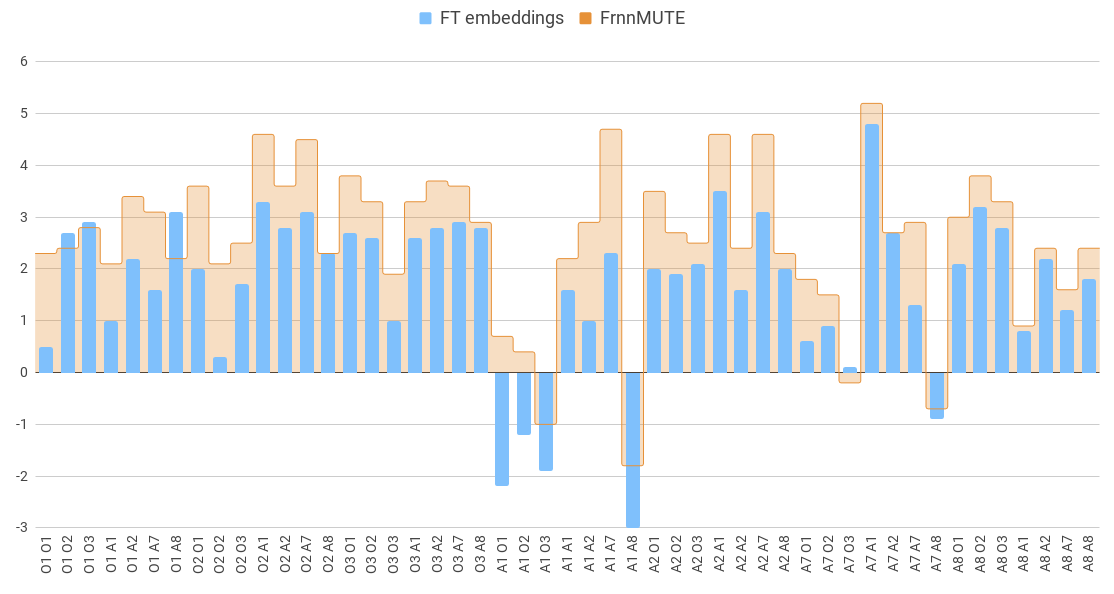
\includegraphics[width=15cm]{Images/f1-diff-frnnmute-ft.png}
    \caption{The difference of F1 score received for user pairs with a classification model built on combination of features (standard and based on deep learning) and on only standard features. }
    \label{fig:f1-diff-frnnmute-ft}
\end{figure} 

\begin{table*}
  \centering
  \begin{tabular}{c|c|c|c|c||c|c|c||c|c|c}
    \multirow{2}{0.6cm}{\textit{Train user}} & \multirow{2}{0.6cm}{\textit{Test user}}  & \multicolumn{3}{L||}{\it Standard features} & \multicolumn{3}{L||}{\it FrnnMUTE} & \multicolumn{3}{L}{\it Standard features + FrnnMUTE}\\ \cline{3-11} 
  &  & $P$ & $R$ & $F$ & $P$ & $R$ & $F$ & $P$ & $R$ & $F$
  \\ \hline
$O1$&$O1$&\he{77.2}&\he{82.5}&\he{79.7}&\he{76.1}&\he{81.0}&\he{78.4}&\he{79.3}&\he{84.9}&\he{82.0}\\
$O1$&$O2$&\he{78.6}&\he{81.7}&\he{80.1}&\he{78.8}&\he{80.7}&\he{79.6}&\he{82.2}&\he{82.9}&\he{82.5}\\
$O1$&$O3$&\he{81.2}&\he{85.0}&\he{83.0}&\he{80.7}&\he{82.6}&\he{81.3}&\he{85.3}&\he{86.5}&\he{85.8}\\
$O1$&$A1$&\he{71.0}&\he{74.7}&\he{71.2}&\he{71.4}&\he{74.5}&\he{71.5}&\he{75.0}&\he{75.7}&\he{73.3}\\
$O1$&$A2$&\he{70.6}&\he{78.4}&\he{74.0}&\he{72.0}&\he{77.3}&\he{73.6}&\he{76.5}&\he{80.2}&\he{77.4}\\
$O1$&$A7$&\he{72.6}&\he{77.5}&\he{74.2}&\he{74.4}&\he{78.1}&\he{75.2}&\he{77.5}&\he{79.4}&\he{77.3}\\
$O1$&$A8$&\he{82.3}&\he{84.9}&\he{83.5}&\he{81.2}&\he{82.2}&\he{81.5}&\he{85.5}&\he{85.8}&\he{85.7}\\
\hline
$O2$&$O1$&\he{77.0}&\he{82.2}&\he{79.1}&\he{77.4}&\he{82.3}&\he{79.5}&\he{82.0}&\he{85.4}&\he{82.7}\\
$O2$&$O2$&\he{78.9}&\he{82.0}&\he{80.0}&\he{76.1}&\he{79.3}&\he{77.6}&\he{80.8}&\he{83.9}&\he{82.1}\\
$O2$&$O3$&\he{81.1}&\he{85.4}&\he{83.0}&\he{79.6}&\he{83.1}&\he{81.2}&\he{84.6}&\he{87.5}&\he{85.5}\\
$O2$&$A1$&\he{71.1}&\he{72.1}&\he{68.2}&\he{71.3}&\he{73.7}&\he{70.1}&\he{74.8}&\he{76.2}&\he{72.8}\\
$O2$&$A2$&\he{70.8}&\he{77.3}&\he{72.7}&\he{72.9}&\he{77.4}&\he{73.1}&\he{76.4}&\he{80.5}&\he{76.3}\\
$O2$&$A7$&\he{72.7}&\he{75.6}&\he{71.8}&\he{73.9}&\he{77.1}&\he{73.7}&\he{76.9}&\he{79.6}&\he{76.3}\\
$O2$&$A8$&\he{83.0}&\he{86.2}&\he{84.4}&\he{81.5}&\he{83.8}&\he{82.4}&\he{85.8}&\he{88.1}&\he{86.7}\\
\hline
$O3$&$O1$&\he{77.4}&\he{82.8}&\he{79.7}&\he{78.9}&\he{82.5}&\he{80.0}&\he{82.5}&\he{85.8}&\he{83.5}\\
$O3$&$O2$&\he{79.0}&\he{82.2}&\he{80.2}&\he{79.0}&\he{81.3}&\he{79.7}&\he{82.9}&\he{84.7}&\he{83.5}\\
$O3$&$O3$&\he{81.2}&\he{85.5}&\he{83.2}&\he{77.0}&\he{80.6}&\he{78.7}&\he{85.4}&\he{87.3}&\he{85.1}\\
$O3$&$A1$&\he{71.8}&\he{73.3}&\he{69.5}&\he{72.6}&\he{72.8}&\he{69.4}&\he{75.5}&\he{75.9}&\he{72.8}\\
$O3$&$A2$&\he{71.2}&\he{78.0}&\he{73.5}&\he{74.0}&\he{77.1}&\he{73.1}&\he{77.2}&\he{80.8}&\he{77.2}\\
$O3$&$A7$&\he{73.2}&\he{76.5}&\he{72.9}&\he{74.5}&\he{76.3}&\he{73.1}&\he{77.6}&\he{79.4}&\he{76.5}\\
$O3$&$A8$&\he{82.6}&\he{85.8}&\he{84.1}&\he{81.4}&\he{83.6}&\he{82.3}&\he{86.2}&\he{88.0}&\he{87.0}\\
\hline
$A1$&$O1$&\he{77.2}&\he{82.5}&\he{79.8}&\he{78.4}&\he{80.6}&\he{78.7}&\he{80.2}&\he{82.4}&\he{80.5}\\
$A1$&$O2$&\he{78.6}&\he{81.6}&\he{80.1}&\he{78.3}&\he{79.1}&\he{78.3}&\he{80.6}&\he{81.2}&\he{80.5}\\
$A1$&$O3$&\he{81.2}&\he{84.9}&\he{82.9}&\he{80.2}&\he{80.2}&\he{79.3}&\he{82.8}&\he{82.9}&\he{81.9}\\
$A1$&$A1$&\he{70.9}&\he{74.7}&\he{71.3}&\he{70.0}&\he{73.5}&\he{70.4}&\he{71.5}&\he{76.8}&\he{73.5}\\
$A1$&$A2$&\he{70.5}&\he{78.3}&\he{74.0}&\he{73.4}&\he{77.4}&\he{73.8}&\he{76.6}&\he{80.4}&\he{76.9}\\
$A1$&$A7$&\he{72.6}&\he{77.5}&\he{74.2}&\he{74.9}&\he{78.7}&\he{76.0}&\he{78.1}&\he{81.5}&\he{78.9}\\
$A1$&$A8$&\he{82.2}&\he{84.8}&\he{83.5}&\he{80.3}&\he{79.7}&\he{79.3}&\he{82.7}&\he{82.1}&\he{81.7}\\
\hline
$A2$&$O1$&\he{77.3}&\he{82.6}&\he{79.8}&\he{79.6}&\he{81.7}&\he{80.5}&\he{82.4}&\he{84.5}&\he{83.3}\\
$A2$&$O2$&\he{78.6}&\he{81.6}&\he{80.1}&\he{79.4}&\he{79.9}&\he{79.6}&\he{82.7}&\he{83.0}&\he{82.8}\\
$A2$&$O3$&\he{81.2}&\he{84.9}&\he{83.0}&\he{81.3}&\he{81.7}&\he{81.2}&\he{85.2}&\he{85.9}&\he{85.5}\\
$A2$&$A1$&\he{70.9}&\he{74.6}&\he{71.2}&\he{73.9}&\he{75.4}&\he{73.3}&\he{77.4}&\he{77.7}&\he{75.8}\\
$A2$&$A2$&\he{70.6}&\he{78.4}&\he{74.0}&\he{72.1}&\he{75.7}&\he{71.6}&\he{76.4}&\he{80.3}&\he{76.4}\\
$A2$&$A7$&\he{72.6}&\he{77.5}&\he{74.2}&\he{75.6}&\he{78.1}&\he{76.1}&\he{79.1}&\he{80.6}&\he{78.8}\\
$A2$&$A8$&\he{82.2}&\he{84.8}&\he{83.4}&\he{81.8}&\he{81.5}&\he{81.4}&\he{85.8}&\he{85.6}&\he{85.7}\\
\hline
$A7$&$O1$&\he{77.1}&\he{82.5}&\he{79.7}&\he{79.1}&\he{81.1}&\he{79.2}&\he{80.9}&\he{83.7}&\he{81.5}\\
$A7$&$O2$&\he{78.5}&\he{81.6}&\he{80.0}&\he{78.7}&\he{79.3}&\he{78.6}&\he{81.1}&\he{82.4}&\he{81.5}\\
$A7$&$O3$&\he{81.0}&\he{84.9}&\he{82.9}&\he{80.5}&\he{80.5}&\he{79.6}&\he{82.9}&\he{84.0}&\he{82.7}\\
$A7$&$A1$&\he{71.0}&\he{74.4}&\he{70.9}&\he{72.5}&\he{76.3}&\he{73.4}&\he{75.1}&\he{79.1}&\he{76.1}\\
$A7$&$A2$&\he{70.5}&\he{78.2}&\he{73.8}&\he{73.1}&\he{77.4}&\he{73.8}&\he{75.6}&\he{80.4}&\he{76.5}\\
$A7$&$A7$&\he{72.6}&\he{77.4}&\he{74.0}&\he{70.4}&\he{76.1}&\he{73.1}&\he{74.3}&\he{80.1}&\he{76.9}\\
$A7$&$A8$&\he{81.9}&\he{84.7}&\he{83.3}&\he{80.5}&\he{80.0}&\he{79.6}&\he{83.0}&\he{83.3}&\he{82.6}\\
\hline
$A8$&$O1$&\he{77.0}&\he{82.4}&\he{79.6}&\he{78.2}&\he{82.4}&\he{79.6}&\he{81.8}&\he{85.3}&\he{82.6}\\
$A8$&$O2$&\he{78.4}&\he{81.5}&\he{79.8}&\he{79.3}&\he{81.9}&\he{80.2}&\he{82.9}&\he{85.2}&\he{83.6}\\
$A8$&$O3$&\he{80.9}&\he{84.9}&\he{82.8}&\he{80.9}&\he{83.7}&\he{81.7}&\he{85.0}&\he{88.1}&\he{86.1}\\
$A8$&$A1$&\he{71.0}&\he{74.2}&\he{70.7}&\he{72.0}&\he{73.1}&\he{69.5}&\he{74.5}&\he{75.2}&\he{71.6}\\
$A8$&$A2$&\he{70.4}&\he{78.1}&\he{73.7}&\he{73.1}&\he{77.3}&\he{72.9}&\he{75.5}&\he{80.4}&\he{76.1}\\
$A8$&$A7$&\he{72.6}&\he{77.2}&\he{73.7}&\he{73.5}&\he{76.5}&\he{73.0}&\he{76.2}&\he{78.7}&\he{75.3}\\
$A8$&$A8$&\he{81.9}&\he{84.9}&\he{83.4}&\he{78.0}&\he{81.2}&\he{79.5}&\he{84.3}&\he{87.5}&\he{85.8}\\
\end{tabular}
  \caption{Detailed study of FrnnMUTE’s performance for words understandibility detection.}
  \label{tab:frnnmute-details}
\end{table*}


\begin{table}[h]
\centering
\begin{tabular}{L|MMM}
\hline
$\mu$ +/- $\sigma$ & user-in vocabulary-out & user-out vocabulary-in & user-out vocabulary-out \\ \hline
Standard features & 78 +/- 4.8 & 77.7 +/- 4.9 & 77.6 +/- 4.9 \\[10pt]
FT emb & 68.1 +/- 5.2 & 67.6 +/- 5.3 & 67.3 +/- 5.2 \\[10pt]
FrnnMUTE & 75.6 +/- 3.8 & 77.1 +/- 3.9 & 74.5 +/- 3.9 \\[10pt]
Standard features + FT emb & 79.1 +/- 4.7 & 79.5 +/- 4.6 & 77.1 +/- 4.6 \\[10pt]
Standard features + FrnnMUTE & 80.3 +/- 4.7 & 80.3 +/- 4.3 & 78.6 +/- 4.4 \\[10pt]
Standard features + FT emb + FrnnMUTE & 80.2 +/- 4.6 & 80.4 +/- 4.3 & 78.1 +/- 4.3 \\ \hline
\end{tabular}
  \caption{Study of our FrnnMUTE's performance for words understandibility detection. For words categorization with Only standard features/ Only FastText word embeddings/ Only FrnnMUTE a decision tree of depth 4 was trained. On all the rest of feature sets a decision tree of depth 9 was trained.}
  \label{tab:frnnmute}
\end{table}


\todo[inline]{you should add a discussion addressing the limitations of your work.}